\documentclass[11pt,singlecolumn]{scrartcl}
\usepackage[bachelorthesis]{systems-cover}
\usepackage{amsmath,amssymb,amstext}
\usepackage[utf8]{inputenc}
\usepackage[english]{babel}
\usepackage{fancyhdr}
\usepackage{graphicx}
\usepackage[capposition=bottom]{floatrow}
\usepackage{pdfpages} 
\pagestyle{fancy}
\fancyhf{}
\fancyhead[LE,RO]{Druid vs. AIM}
\fancyhead[RE,LO]{Lukas Striebel}

\fancyfoot[RE,lO]{Bachelor Thesis}
\fancyfoot[LE,RO]{\thepage}

\renewcommand{\headrulewidth}{2pt}
\renewcommand{\footrulewidth}{1pt}

\covernum{132 b}
\covertitle{Druid vs. AIM\\[1cm]A comparison of two real-time analytical data storage systems}
\coverauthor{Lukas Striebel}
\coverdate{09.02.2015 - 09.07.2015}
\coversupervisedby{Prof.\ Donald Kossmann, Lucas Braun, Renato Marroquin}




\begin{document}
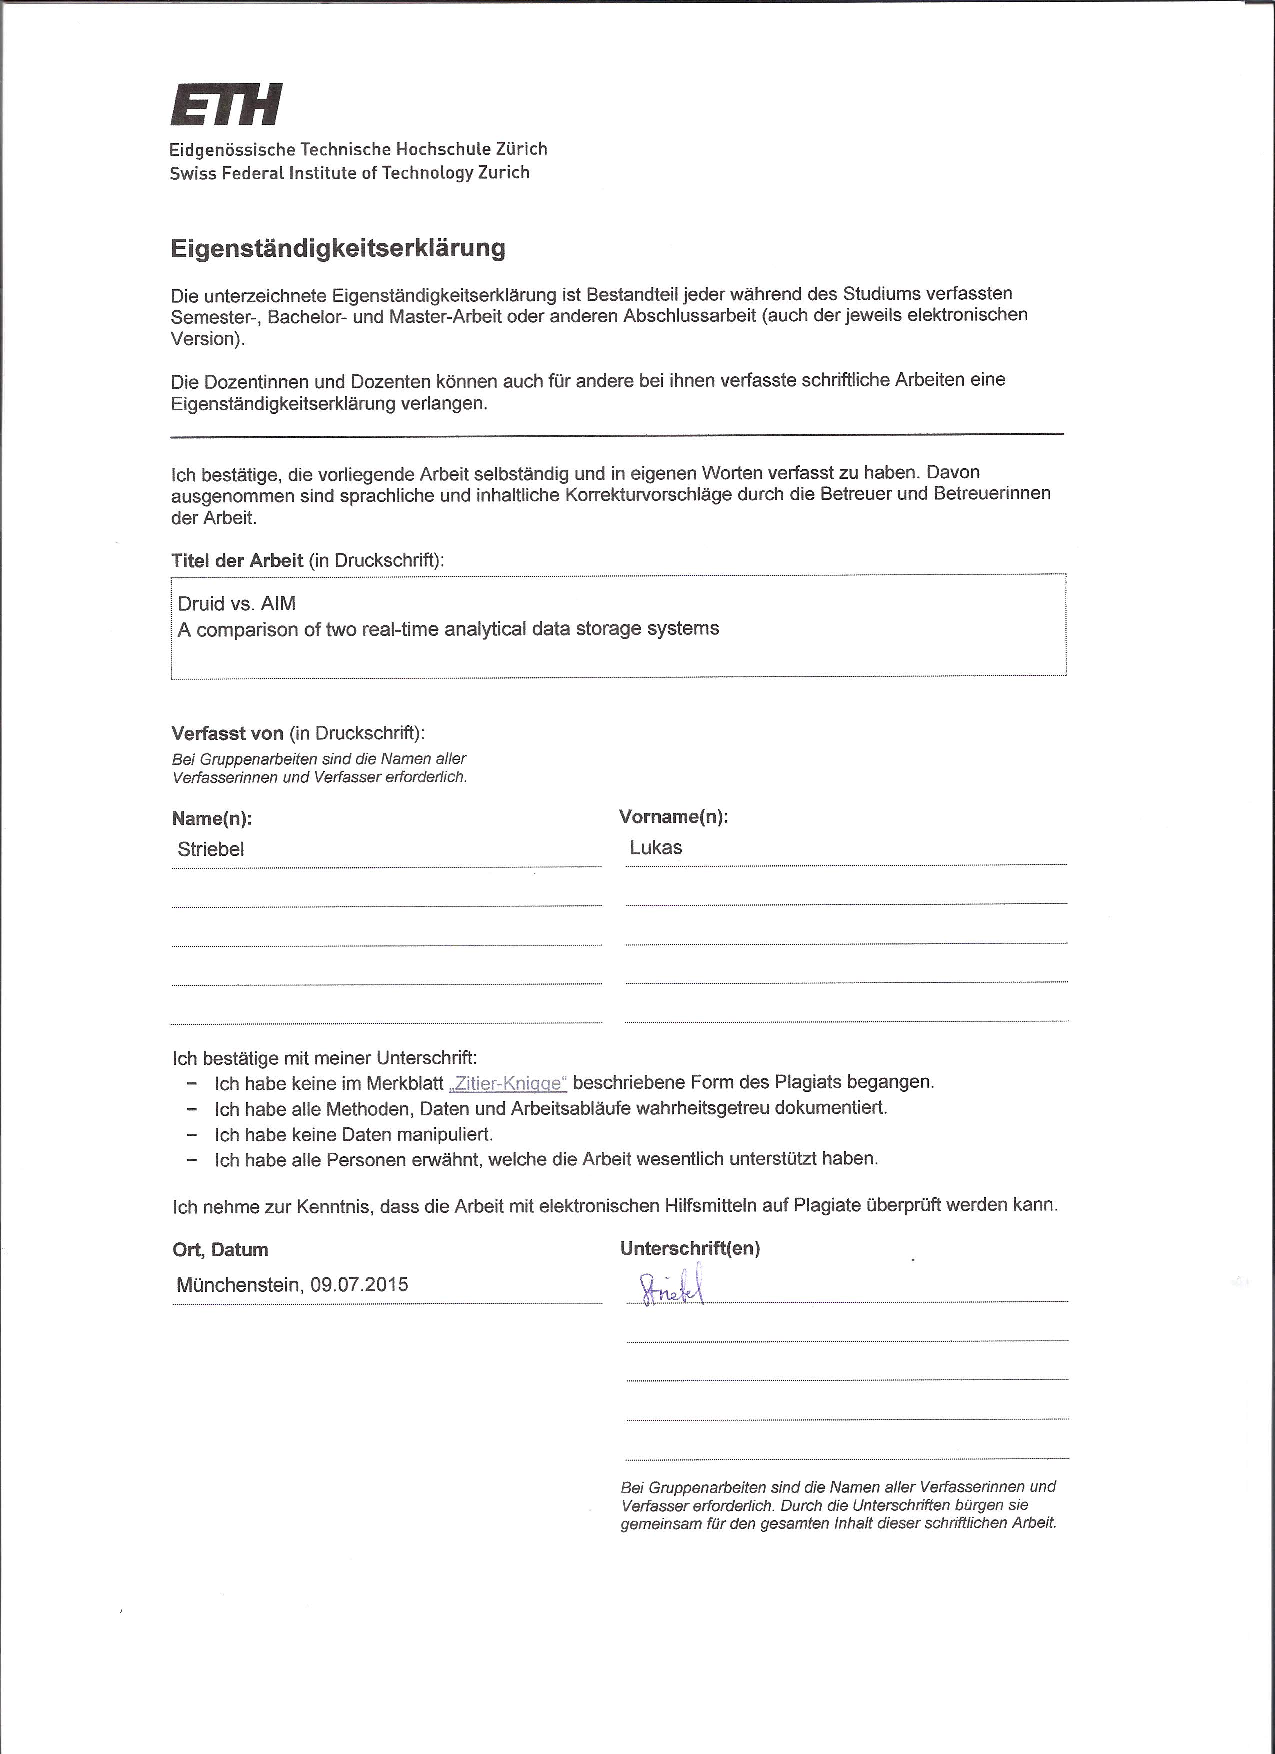
\includepdf[pages={1}]{eig.pdf}
\hspace{60mm}
\begin{center}
 \textbf{Abstract} \end{center}


In today's society, data is arguably one of the most valuable goods. In recent years, many data related research fields have thrived: Big data and advanced analytics, health IT and Bioinformatics, data protection and encryption, just to name a few. Dealing with huge amount of data is without doubt essential for any company. In this thesis two different data stores, AIM and Druid, are compared against each other. The thesis further explores how these two system could be used together in order to support each other. Our experiments have shown promising results and suggest that Druid may indeed serve as a proper backup system for AIM.


\clearpage
\tableofcontents
\clearpage
\section{Introduction}
\subsection{Motivation}
As of 2015, the number of mobile devices has officially surpassed the world's population \cite{ind}. Every day, billions of phone calls are made and billions of text messages are sent. Use of mobile phones has become an essential part of our daily routine. This development has led to unprecedented proliferation and growth of telecommunication companies. These companies are in constant competition to provide the best possible service to their customers, as well as maintaining high profits.\\\\\\One of the many challenges those companies have to address is to deploy a suitable storage system for their users' data and call histories. Scalability and efficiency are only two of the many requirements such a system must fulfill. Data stores which are capable of dealing with these challenges are in high demand. The goal of this thesis is to compare two different databases, Druid and AIM, in a realistic environment. In addition, we will lay out how the two system can be used together in order to complement each other and compensate each other's weaknesses.\\[1 cm]



\subsection{Thesis Structure}
The thesis is structured as follows. In Section 2 the Druid and AIM systems are introduced and the benchmark is explained. Section 3 contains the different approaches, some successful and some unsuccessful, on how to run this benchmark on Druid. The obtained results are discussed in section 4. Section 5 summarizes my conclusions and provides an outlook.
\clearpage

\section{Background}
\subsection{The AIM Architecture}
The AIM system \cite{aim} is currently being developed at ETHZ by various people. It is designed for storing large amounts of data as well as dealing with synchronous updates and queries. A possible use case would e.g. be a telecommunications company where telephone calls would constitute the database entries. Queries would be needed to retrieve specified call statistics for individual customers or customer groups, e.g. average call duration, number of calls within a specified period, and so on. A basic overview of the AIM architecture is displayed in Figure 1.\\\\

\begin{figure}[h]
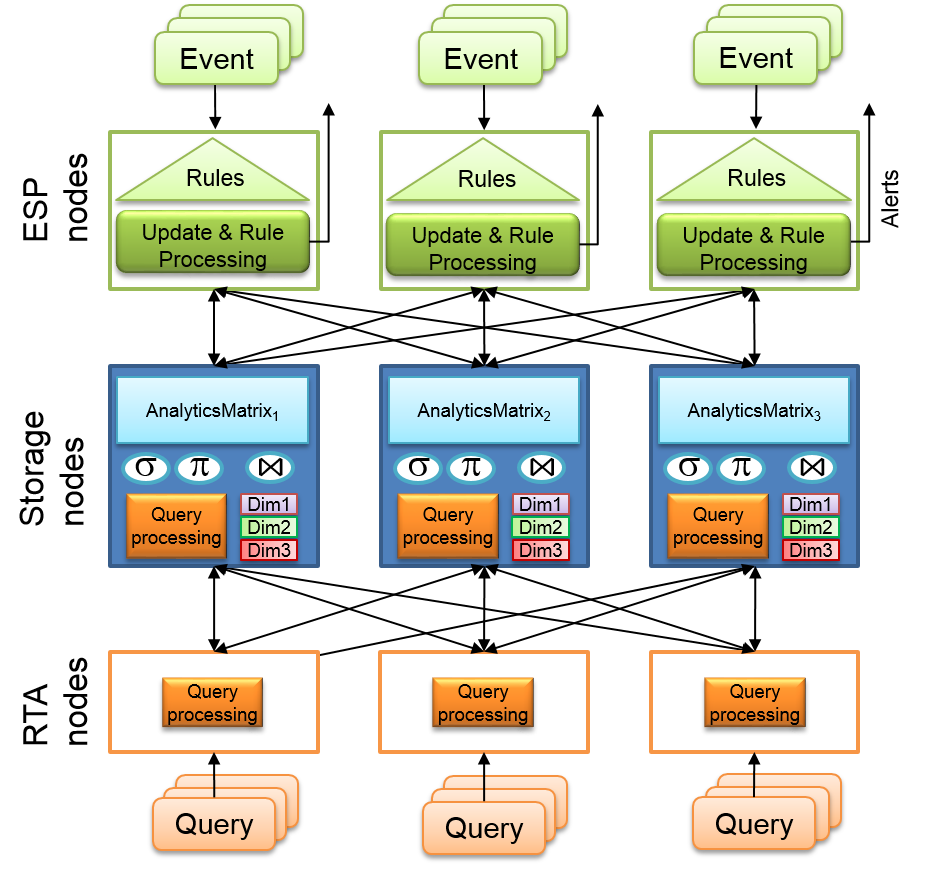
\includegraphics[scale=0.7]{layers.png}
\caption{The AIM architecture, graphic taken from \cite{aim}}
\end{figure}
\vspace{10mm}
The core idea behind AIM is to have two separate parts, the SEP and the RTA, to handle the different challenges.  Both parts operate on a large amount of data, called the \textit{Analytics Matrix}, which can be imagined as a very large and wide table. \\\\The \textit{Stream Event Processing} (SEP)  receives updates and modifies the Analytics Matrix accordingly. Incoming updates are stored inside a buffer which periodically merges into main storage. This mechanism is called \textit{Differential Updates}. Every time an update is executed, a set of \textit{Business Rules} is evaluated, checking if a customer is eligible for certain special offers. For example, a company might offer specific discounts for highly active users.\\\\ Due to its size, the Analytics Matrix is usually not stored on a single machine, but instead distributed amongst multiple data storage nodes. AIM uses a shared nothing architecture and stores its data in a column oriented memory structure called \textit{ColumnMap}. The \textit{Real-Time Analytics Processing} (RTA) is responsible for processing the queries and assembling the partial results received from the various distributed data storage nodes.

\clearpage

\subsection{The Druid Architecture}
Developed by Metamarkets Inc., the Druid system \cite{druid} is built on four different types of nodes each of which fulfilling one of these tasks: Data ingesting, storing, querying and coordinating. Both the Overlord node and the Realtime node are responsible for the data ingestion. The difference between them is that the Realtime node is used in case of a continuous data stream, e.g. Amazon sales data whereas the Overlord node is used whenever the data to be ingested is already known, as is the case in the AIM benchmark.\\
The Historical node saves the ingested data segments on Deep Storage which can be a hard disk, Amazon S3 or whatever else is specified.\\
The Broker node directs incoming queries to the corresponding Historical node.\\
The Coordinator nodes in combination with Zookeeper \cite{zoo} manages the interactions between the different nodes.\\


\begin{figure}[h]
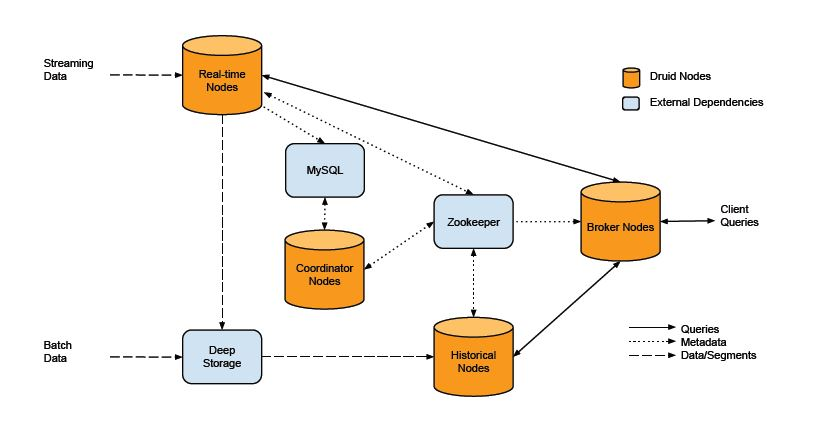
\includegraphics[scale=0.65]{druid.jpg}
\caption{The Druid architecture, graphic taken from \cite{druid}}
\end{figure}

There are a number of extensions compatible with Druid, most notably Apache Hadoop \cite{hadoop} which will be used later on in this thesis. Hadoop on its own is a powerful distributed data storage and processing framework. However in our case we will only use it to replace the Overlord node in our Druid system. As stated by the developers and verified by personal experience, the Overlord node works efficiently only as long as the size of the data file is below 1 GB. After exceeding this threshold, performance drops significantly. We therefore used a single Hadoop node for the ingestion of larger files.
\\[1cm]
Druid is open source and currently available at \cite{druidon}.

\clearpage

\subsection{The original Benchmark}
For the benchmark, we were using the mentioned example of a large telephone company with millions of subscribers, also referred to as customers. The original benchmark consisted of two parts, one for the RTA and another for the SEP. The Analytics Matrix was set up to contain a total of ten million subscribers. Each customer was described with 42 unique attributes such as number of calls or longest call duration. These 42 attributes were duplicated 13 times in order to create a more realistic and challenging environment. This resulted in a total amount of 546 attributes per subscriber.\\\\
In the first part of the benchmark, the performance of the SEP was evaluated. Three million updates, each one relating to a single subscriber, were applied to the Analytics Matrix and the elapsed time was measured.\\\\In the RTA part, the performance for answering seven different SQL queries, featuring various Joins and Aggregations, was measured. 
\clearpage

\section{Methods}

\subsection{First Attempts}
In our first attempts we tried to implement exactly the same AIM benchmark on Druid. This meant that Druid had to store only one row for each customer, which contained various static attributes such as subscriber-ID, cheapest call this week etc., as well as the entire 546 aggregations, resulting in a very wide table. However, it also yielded the benefit of having a table of constant size, rather than an ever growing one. Approaching the benchmark this way greatly simplified the RTA part. Since Druid does not understand SQL, the only thing to do was to translate the original seven queries into a format that Druid was able to understand.\\\\
However, it soon became clear that updating existing data in Druid is quite difficult, since Druid does not feature any kind of native updating functionality. Instead it is suggested to simply ingest a new, more up-to-date record which would overwrite the existing one. Therefore the only possible way to execute an update in the sense of the SEP benchmark would be to send a query to retrieve the old record, manually update it and then re-ingest that record. Unsurprisingly, this approach performed very poorly. As we did not find a more elegant solution to update the records in Druid, we decided to abandon this original benchmark and to take a different path.    
\\[0.6 cm]

\subsection{Rethinking the benchmark}
As AIM lacks a reliable recovery system, we decided to instead test whether Druid could be used as a suitable backup system for AIM. This implied that Druid now was used to save all the calls rather than all the subscribers. In case of a critical failure of AIM, would it be possible to reconstruct the customers' call data using the Druid backup, in a reasonable time period?\\\\
Storing the calls instead of the users' data presented a set of new challenges. One of our main concerns was scalability, since the number of calls increases substantially faster than the number of subscribers. Would Druid be able to deal with such a rapidly growing database?\\\\We decided to focus on three major points in our benchmark:
\begin{itemize}

 \item The \textbf{ingestion rate}, measured in rows/second and kB/second
 \item The time it takes to restore all attributes for every customer (\textbf{full restore})
 \item The time it takes to restore all attributes for a single customer (\textbf{single restore})
\end{itemize}
We set up our experiments to verify whether these values stayed within an acceptable magnitude, even if the number of calls grows very large. In order to prove this point, we decided to let Druid consecutively ingest 10 segments of data, and send a set of queries after each data segment. Every segment was 120 MB large and contained 1'048'576 rows of phone calls. Each phone call was described using five attributes:
\begin{itemize}

 \item  The time stamp
 \item  The subscriber-ID, ranging from 1 to 1'000'000
 \item  The call duration, ranging from 1 to 10'000
 \item  The cost of the call, ranging from 1.0 to 99.9
 \item  A boolean to indicate whether the call was local or non-local
\end{itemize}
Each query would then reconstruct one of the original 42 attributes, e.g. the sum of a subscriber's call durations, the longest call this week etc. Measuring the ingestion rate as well as the time it takes for these queries to complete should give us an idea whether or not Druid is eligible to act as a backup system for AIM. 

\clearpage


\section{Results and Discussion}
\subsection{Small Benchmark}As mention in Section 3, the three domains under measurement were the ingestion rate, the full restore and the single restore. However, we were more interested in their development over the course of the benchmark rather than the actual values. As the database grew larger, from 1 million rows after the first segment up to 10 millions after the last one, the amount of time for a full restore was expected to increase, whereas the time for the ingestion and the single restore should stay constant to some degree.\\\\The first successful benchmark was run on a private machine with 7.8 GB of memory and an Intel Core i7-2600 CPU @3.4 GHz x 8, using Ubuntu 14.04 LTS 64-bit. (See Figure 3)

\begin{figure}[h]
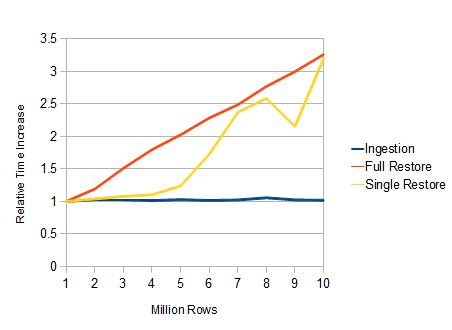
\includegraphics[scale=1.1]{loc.jpg}
\caption{Small Benchmark on a private machine}
\end{figure}


In this diagram, the relative time in- or decrease over the course of the benchmark  \textbf{in relation to the very first segment}, is displayed. The development shows a nearly constant ingestion rate, as expected. Ingesting a single segments took 124 seconds on average, resulting in a rate of 8460 rows/second or 947 kB/second. These results were unsurprising and met the expectations.\\\\\\
However, the single restore behaved oddly. Later experiments indicated that the results likely were disturbed by extreme outliers. The results of the subsequent benchmarks support this claim.\\\\
Unfortunately, Druid was not able to restore the full Analytics matrix in a single query. All such attempts ended in a time-out failure. In order to overcome this problem, we split the subscribers in 10 smaller groups, according to their IDs. This step resolved the problem and we were able to obtain reasonable results.
As the graphic shows the query times increased only linearly and not exponentially. After the 10th segment, the full restore was 3.5 times slower than after the first. These times were acceptable, considering the amount of data had increased by a factor of 10. 
\\[1cm]
The same benchmark was also run on Euler07, a machine with 129 GB RAM  and an Intel Xeon CPU E5-2609 @ 2.40GHz x 8, using a Linux kernel 3.18.\\
These following results were obtained. (See Figure 4)  

\begin{figure}[h]
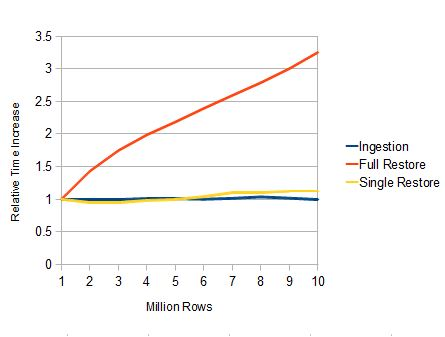
\includegraphics[scale=1.1]{eul.jpg}
\caption{Small Benchmark on the Euler07}
\end{figure}


Again, the diagram depicts the relative time in- or decreases of the 3 fields under measurement. The ingestion rate and the full restore behaved almost identical to the other benchmark, remaining constant resp. increasing up to a factor 3.5.\\\\Despite the enormous gain of memory, the ingestion rate did not improve. It actually decreased down to 6'520 rows/second resp. 747 kB/second. This indicates that the ingestion was primarily capped by the CPU, which is not surprising.\\\\On the other hand, the absolute times for the full restore decreased significantly, as apparently querying is capped by memory.\\\\
The interesting point to notice is the single record restore, which remained constant, in contrast to the previous benchmark. The absolute times for the single restore after the first segment remained unchanged in comparison to the other benchmark.


\clearpage
\subsection{Hadoop for Big Data}
In order to create a more realistic test environment, we increased the size of each data segment by a factor 10. The separate files now contained 10'485'760 rows each and were 1.2 GB large. In order to ingest these large datasets, we set up a single Hadoop node, rather than relying on the Overlord node. Besides these changes the benchmark remained the same. The following results were obtained on the same private machine as in section 4.1. (See Figure 5) 

\begin{figure}[h]
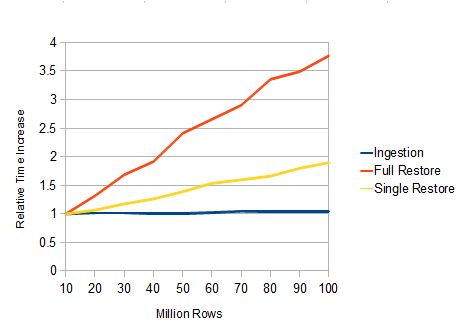
\includegraphics[scale=1.1]{100m.jpg}
\caption{Large Benchmark on a private machine}
\end{figure}

Once again, the ingestion rate remained more or less constant throughout the entire benchmark. It took Druid resp. Hadoop 689 seconds on average to complete the task, which results in an ingestion rate of 15'200 rows/second or 1'740 kB/second. The development of the query times is similar to the small benchmark on the Euler machine, although they executed a lot slower due to the increased size of the database. The elapsed times for the full restore increase linearly up to a factor 4. The single restore slows down slightly, up to a factor 2. \\\\
In all three benchmarks the initial ingestion rate remained constant and the query times increased only linearly, up to a factor 4 for the full restore resp. a factor 2 for the single restore. These results met the expectations and proved the scalability of our Druid-AIM setup. 

\clearpage
\section{Summary}
\subsection{Conclusion}
Motivated by use cases from the telecommunications industry, we attempted to put the performance of two promising data stores, Druid and AIM, into perspective. Having already a realistic and challenging test environment for AIM at hand, we tried to execute the exact same benchmark on Druid. However, it soon became clear that such a comparison makes little sense, since the two systems are designed for completely different purposes. Druid excels at ingestion of a huge continuous stream of data while having trouble updating existing data, which is one of the core strengths of AIM.\\\\\\
Rather than heavily modifying the AIM benchmark, we came up with a new one which was supposed to verify Druid's suitability as a backup store for AIM, as AIM currently lacks the ability to restore its content in case of severe failure. The obtained results indicate that this is indeed the case, as Druid's ingestion rate remained constant, and the query times increased only linearly which is acceptable.\\\\\\
The original goal of this thesis was to execute the AIM-benchmark on Druid, which we unfortunately were unable to achieve. However, we were able to demonstrate that the collaboration of the two system shows promising results. It remains to be seen whether Druid and AIM are able to assert themselves in the huge and competitive field of data stores. There are countless competitors, such as Impala, Cassandra or Hadoop, and it would be interesting to see how they fare in direct comparison. However, this is material for future work.

\subsection{Acknowledgements}
I would like to thank my supervisors Lucas Braun and Renato Marroquín for their continuous support and help. They provided many meaningful suggestions and proposals. Their expertise and experience was invaluable.\\\\
I would also like to thank Professor Kossmann for taking the time to supervise my thesis.\\\\
A special thanks thanks goes to my parents for keeping me motivated and for reviewing this thesis.

\clearpage

\begin{thebibliography}{1}
\bibitem {druid} Fangjin Yang, Eric Tschetter, Xavier Léauté, Nelson Ray, Gian Merlino, Deep Ganguli.
{\em Druid. A Real-time Analytical Data Store}, In: Proceedings of the 2014 ACM SIGMOD International Conference on Management of Data, pp. 251 - 264

\bibitem{aim} Lucas Braun, Thomas Etter, Georgios Gasparis,
Martin Kaufmann, Donald Kossmann, Daniel Widmer, Aharon Avitzur, Anthony Iliopoulos, Eliezer Levy, Ning Liang.
{\em Analytics in Motion. High Performance Event-Processing AND Real-Time Analytics in the Same Database}, In: Proceedings of the 2015 ACM SIGMOD International Conference on Management of Data, pp. 157-168

\bibitem{druidon}
Metamarkets Inc. {\em Druid.} http://druid.io/, 2014. [Online; accessed July 2015].

\bibitem{hadoop}Apache Foundation. {\em Hadoop.} http://hadoop.apache.org/, 2013. [Online; accessed July 2015].

\bibitem{zoo}Apache Foundation. {\em Zookeeper.} http://zookeeper.apache.org/, 2014. [Online; accessed July 2015].

\bibitem{ind} The Independent. {\em There are officially more mobile devices than people in the world.} http://www.independent.co.uk/life-style/gadgets-and-tech/news/there-are-officially-more-mobile-devices-than-people-in-the-world-9780518.html, 2014. [Online; accessed July 2015].

\end{thebibliography}

\end{document}